\chapter{Metodi di ricerca sistematici} \label{ch:Metodi di ricerca sistematici}
\section{Metodi di ricerca sistematici}
I CSP sono problemi combinatori, quindi si deve trovare una soluzione su tutte le possibili combinazioni di assegnamenti che si possono avere in maniera tale da soddisfare tutti i vincoli. I vari metodi per fare questo sono:
\begin{enumerate}
    \item \textbf{Generate and Test: }Probabilmente il metodo di risoluzione dei problemi più generale. L’algoritmo consiste nei seguenti due passaggi che si ripetono:
    \begin{enumerate}
        \item si generano le etichette
        \item si controlla se vanno bene gli assegnamenti.
    \end{enumerate}
    Alcuni possibili miglioramenti sono ad esempio uno smart generator, ovvero si assegnano i valori alle variabili e se non vanno bene si effettuano dei cambiamenti sugli assegnamenti errati (ricerca locale). Un altro miglioramento consiste nel fare il test sugli assegnamenti e poi fare backtracking.
    \item \textbf{Check and Instantiate: }Assegno uno alla volta i valori alle variabili verificando di non violare i vincoli presenti.
    \item \textbf{Backtraking:} Assegno uno alla volta i valori alle variabili finchè non violo un vincolo; appena lo violo, torno indietro nell’assegnamento. Si estende quindi una soluzione parziale verso una soluzione completa.
\end{enumerate}
\newpage
\subsection{Backtraking}
Supponiamo di avere un problema CSP con 4 variabili (A,B,C,D), supponiamo che i vincoli siano
\begin{center}
    $A = D, B \neq D, A + C < 4$
\end{center}
L’algoritmo consiste in:
\begin{enumerate}
    \item Assegna il valore alla variabile;
    \item Si controlla la consistenza;
    \item Finchè tutte le variabili sono etichettate;
\end{enumerate}
\begin{figure}[htp]
	\centering
    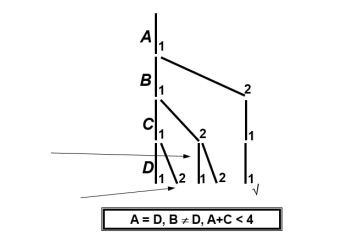
\includegraphics[width=10cm, keepaspectratio]{img/Cap2/back1.png}
    \caption{Esempio backtracking}
\end{figure}
Se tutte le variabili non sono etichettate si torna al passo 1. L’assegnamento delle variabili è commutativo ad esempio
\begin{center}
    $[WA = red$ allora $NT = green]$ come [$NT=green$ allora $WA =red]$
\end{center}
\newpage
Si devono solo considerare gli assegnamenti alle singole variabili per ogni nodo $\rightarrow$ b = d
e ci sono $d^n$ foglie. 
\\La \textbf{DFS} per i CSP son gli assegnamenti a variabili singole è chiamata ricerca \textbf{backtracking}, essa è l’algoritmo base uniformed per i CSP.
\begin{figure}[htp]
	\centering
    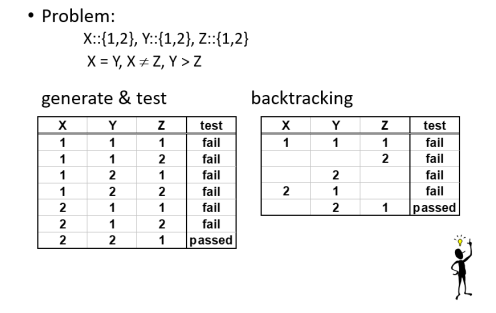
\includegraphics[width=10cm, keepaspectratio]{img/Cap2/back2.png}
    \caption{Esempio generate and test vs backtracking}
\end{figure}
\subsection{Ricerca backtracking: incrementale}
La strategia di ricerca è la \textbf{DFS (Depth First Search):}
\begin{enumerate}
    \item scegli una variabile non istanziata, scegli un valore dal suo dominio, controlla se qualche vincolo è violato;
    \item se nessun vincolo viene violato, continua la ricerca in modo ricorsivo;
    \item altrimenti, torna indietro: torna alla decisione precedente e fai un’altra scelta.
\end{enumerate}
In termini di grandezza dell’albero di ricerca il numero di foglie è pari a $d^n$, dove n è il numero di variabili e $d = max|D_i|$.
\newpage
\begin{figure}[htp]
	\centering
    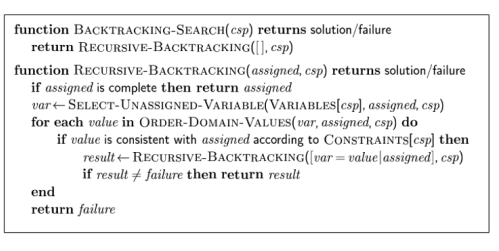
\includegraphics[width=12cm, keepaspectratio]{img/Cap2/dfs.png}
    \caption{Algoritmo di backtracking.}
\end{figure}
\begin{figure}[htp]
	\centering
    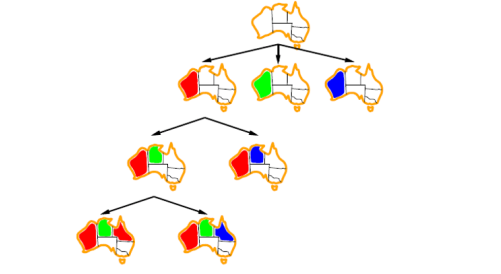
\includegraphics[width=12cm, keepaspectratio]{img/Cap2/dfs2.png}
    \caption{Esempio backtracking.}
\end{figure}
\subsection{Miglioramenti dell’efficienza del backtracking}
Per impostazione predefinita, SELECT-UNASSIGNED-VARIABLE seleziona semplicemente la successiva variabile non assegnata nell’ordine dato dalla lista VARIABLES[csp]. 
\\Questo ordinamento di variabili statiche raramente si traduce nella ricerca più efficiente. 
\\Ad esempio, dopo le assegnazioni per WA = rosso e NT = verde, c’è un solo valore possibile per SA, quindi ha senso assegnare SA = blue next piuttosto che assegnare Q.
\\ Infatti, dopo l’assegnazione di SA, le scelte per Q, NSW e V sono tutte forzate.

\newpage
\textbf{Variabile più vincolata } In questo caso si va a scegliere fra le variabili disponibili per l’assegnamento quella più vincolata in base ad alcune caratteristiche:
\begin{itemize}
    \item si sceglie la variabile con il \textbf{minor numero di valori legali} (minimum remaining values-MRV). È stata anche chiamata la "variabile più vincolata" o euristica "fail-first", quest’ultima perché seleziona una variabile che ha maggiori probabilità di causare un errore presto, potando così l’albero di ricerca.
    \begin{figure}[htp]
    	\centering
        
\includegraphics[width=12cm, keepaspectratio]{img/Cap2/m1.png}
    \end{figure}
    \item si sceglie la variabile con \textbf{più vincoli possibili} (degree heuristic) sulle variabili rimanenti.
    \begin{figure}[htp]
    	\centering
        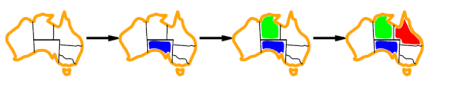
\includegraphics[width=12cm, keepaspectratio]{img/Cap2/m2.png}
    \end{figure}
    \item data una variabile, si sceglie \textbf{il valore meno vincolante} (least-constraining-value), quello che esclude il minor numero di valori nelle restanti variabili.
    \begin{figure}[htp]
    	\centering
        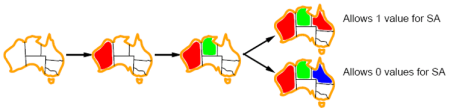
\includegraphics[width=12cm, keepaspectratio]{img/Cap2/m3.png}
    \end{figure}
\end{itemize}
\newpage
\section{Propagazione delle informazioni attraverso vincoli}
Finora il nostro algoritmo di ricerca considera i vincoli su una variabile solo nel momento in cui il variabile viene scelta da SELECT-UNASSIGNED-VARIABLE. Ma guardando alcuni dei vincoli all’inizio della ricerca, o anche prima dell’inizio della ricerca, possiamo drasticamente ridurre lo spazio di ricerca.
\subsection{Forward Checking}
\textbf{Forward Checking: }  Prima di assegnare una variabile controlla che questo assegnamento mi renda possibile futuri assegnamenti ad altri nodi, poichè se dopo l’assegnamento un dominio per una variabile diventasse vuoto, non si avrebbe soluzione e quindi l’assegnamento non andrebbe nemmeno provato.
\\\textbf{Euristica utilizzata: }  Elimina i valori dal dominio quando viene fatto un
assegnamento ad una variabile, se un dominio diventa vuoto, interrompi la ricerca poichè la soluzione non esiste con gli assegnamenti fatti. Questo metodo offre spesso una soluzione senza avere backtrack.
\begin{figure}[htp]
    \centering
    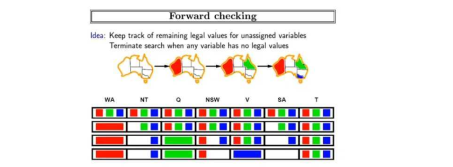
\includegraphics[width=12cm, keepaspectratio]{img/Cap2/f1.png}
\end{figure}
\begin{figure}[htp]
    \centering
    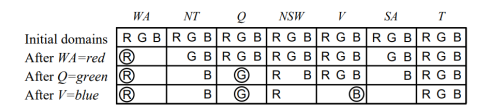
\includegraphics[width=11cm, keepaspectratio]{img/Cap2/f2.png}
    \caption{orward checking applicata a Map-colouring problem.}
\end{figure}
\\Ci sono due punti importanti da notare su questo esempio. Innanzitutto, si noti che dopo aver assegnato WA = rosso e Q = verde, i domini di NT e SA sono ridotti ad un unico valore; abbiamo eliminato del tutto la ramificazione su queste variabili di propagare le informazioni da WA e Q. L’euristica MRV, che è un partner ovvio per il controllo in avanti, selezionerebbe automaticamente SA e NT successivamente.
\subsection{Constraint propagation}
Sebbene il forward checking rilevi molte incoerenze, non le rileva tutte. Per esempio, consideriamo la terza riga della Figura 1.7. Essa mostra che quando WA è rosso e Q è verde, sia NT che SA sono costretti a essere blu ma questo non è possibile perchè sono due zone vicine. Il forward checking non rileva questo come un’incoerenza, perché non guarda abbastanza avanti. La propagazione del vincolo (constraint propagation) è il termine generale per propagare le implicazioni di un vincolo su una variabile su altre variabili; in questo caso dobbiamo propagare da WA e Q su NT e SA, e quindi sul vincolo tra NT e SA per rilevare l’incoerenza.
\section{Grafo delle dipendenze (funzionali)}
Per controllare la correttezza degli assegnamenti viene creato $il$ $grafo$ $delle$ $dipendenze$   $(funzionali)$, dove viene messo un nodo per ogni variabile e un arco tra le variabili che appaiono nello stesso vincolo.
\begin{figure}[htp]
    \centering
    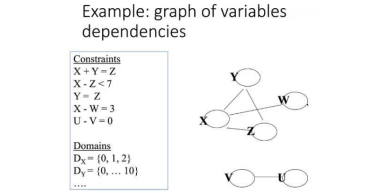
\includegraphics[width=11cm, keepaspectratio]{img/Cap2/grafo-funzionali.png}
    \caption{Esempio grafo delle dipendenze funzionali}
\end{figure}
